\vspace{-3cm}\chapter{实验5. 直方统计图}

\section{5.1 题目}
 
编写一个程序,从文件中读入不定个数的数据。每个数据都已空格或者回车分割,每个数的大小都在[0..100]之间,统计10
个区间的数据的个数,并以两种方式将统计结果进行展示:水平直方图和垂直直方图。示例图如下:(测试数据自行准备)

\begin{figure}[H]
    \centering
    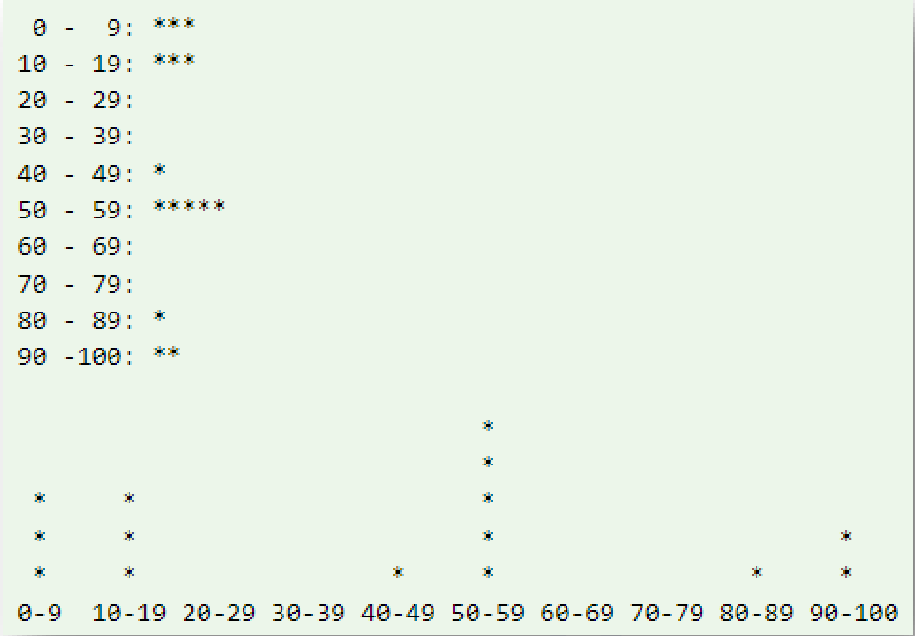
\includegraphics[width = 0.7\textwidth]{../pic/5/5.0.png}
\end{figure}

\section{5.2 思路分析}

本题可分为四个模块。
\begin{enumerate}
    \item \textbf{数据输入}. 为了优雅方便地测试和生成数据,我们采用\lstinline{Random}类批量生成并存储在\lstinline{input/input5.txt}中
        \begin{itemize}
            \item 最常用的是Random中的\lstinline{public int nextInt(int origin, int bound)}这一函数,该函数会返回一个
                [\lstinline{origin}, \lstinline{bound})之间的整数,下文分别简称为上界和下界;
            \item 题目未要求数据的个数。考虑到题目的相关要求,决定把以下界为50,上界为101随机得到一个数据个数;
            \item 每个数据以下界为0,上界为101随机生成,用回车分割并通过\lstinline{BufferedWriter}类(需要
                \lstinline{throw IOException})写入到文件中。
        \end{itemize}
    \item \textbf{数据读取与统计}. 用一个长度为10的整型数组(\lstinline{stat})存储十个部分各自出现的频次。
        \begin{itemize}
            \item 因为数据个数不确定,所以需要\lstinline{hasNext()}确定。
            \item 从文件中读取数据时可以读取每个数据后直接将数据\lstinline{/10},然后将对应的数组中的数\lstinline{+1}。
                需要为100设置一个特例。
        \end{itemize}
    \item \textbf{水平直方图打印}. 对每一行只需在第i行:
        \begin{enumerate}
            \item 打印各自的前缀,第一行和最后一行设置一个特例;
            \item 打印\lstinline{stat[i]}个\lstinline{*}并打印回车;
        \end{enumerate}
    \item \textbf{垂直直方图打印}. 参考Problem4中以像素矩阵的角度打印。
        \begin{enumerate}
            \item 首先遍历数组得到最大值以确定这个矩阵的高度;
            \item 不用把每个打印都看作一个像素,而是把每一部分看作像素,经过这样分割后只需观察每个像素内打印空格的规律;
            \item 对每一行刚开始的时候打印一个空格作为特例,为了保证输出的正确性最后一次打印后即回车;
            \item 最后一行需要输入每个部分的表示。
        \end{enumerate}
\end{enumerate}

\section{5.3 代码与测试}

本题代码完全参照5.2中的思路,实现较为简单,具体可翻阅附录。

本题重在打印出的形式是否正确对应,所以随机打印即可。

\section{5.4 运行结果}

运行结果如下

\begin{figure}[H]
    \centering
    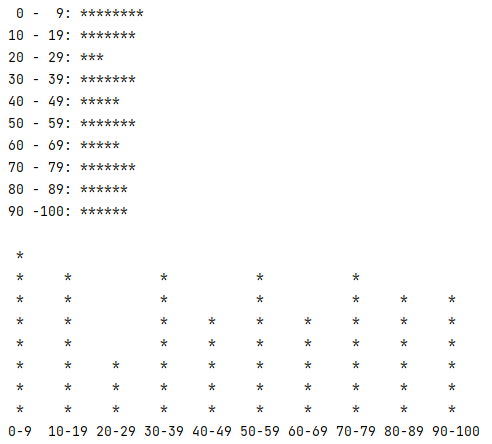
\includegraphics[width = 0.5\textwidth]{../pic/5/5.1.png}
\end{figure}

\section{5.5 总结与收获}

本题比较简单,只是有点繁琐,但需要考虑到设置范围的问题。其次需要从题目给定的样例中总结打印的规律,并把这个规律转换成打印时的一个个单元处理。

第一遍写代码时没有采用\lstinline{hasNext()},运行出现了问题,这说明我对文件输入依旧比较陌生;也没有采用即读即记录,而是打算先存储到
\lstinline{Vector}中,
以后写代码一定要下意识思考优化问题,但也不能看到什么都想到优化。